% Options for packages loaded elsewhere
\PassOptionsToPackage{unicode}{hyperref}
\PassOptionsToPackage{hyphens}{url}
%
\documentclass[
]{article}
\usepackage{amsmath,amssymb}
\usepackage{lmodern}
\usepackage{ifxetex,ifluatex}
\ifnum 0\ifxetex 1\fi\ifluatex 1\fi=0 % if pdftex
  \usepackage[T1]{fontenc}
  \usepackage[utf8]{inputenc}
  \usepackage{textcomp} % provide euro and other symbols
\else % if luatex or xetex
  \usepackage{unicode-math}
  \defaultfontfeatures{Scale=MatchLowercase}
  \defaultfontfeatures[\rmfamily]{Ligatures=TeX,Scale=1}
\fi
% Use upquote if available, for straight quotes in verbatim environments
\IfFileExists{upquote.sty}{\usepackage{upquote}}{}
\IfFileExists{microtype.sty}{% use microtype if available
  \usepackage[]{microtype}
  \UseMicrotypeSet[protrusion]{basicmath} % disable protrusion for tt fonts
}{}
\makeatletter
\@ifundefined{KOMAClassName}{% if non-KOMA class
  \IfFileExists{parskip.sty}{%
    \usepackage{parskip}
  }{% else
    \setlength{\parindent}{0pt}
    \setlength{\parskip}{6pt plus 2pt minus 1pt}}
}{% if KOMA class
  \KOMAoptions{parskip=half}}
\makeatother
\usepackage{xcolor}
\IfFileExists{xurl.sty}{\usepackage{xurl}}{} % add URL line breaks if available
\IfFileExists{bookmark.sty}{\usepackage{bookmark}}{\usepackage{hyperref}}
\hypersetup{
  hidelinks,
  pdfcreator={LaTeX via pandoc}}
\urlstyle{same} % disable monospaced font for URLs
\usepackage[margin=1in]{geometry}
\usepackage{longtable,booktabs,array}
\usepackage{calc} % for calculating minipage widths
% Correct order of tables after \paragraph or \subparagraph
\usepackage{etoolbox}
\makeatletter
\patchcmd\longtable{\par}{\if@noskipsec\mbox{}\fi\par}{}{}
\makeatother
% Allow footnotes in longtable head/foot
\IfFileExists{footnotehyper.sty}{\usepackage{footnotehyper}}{\usepackage{footnote}}
\makesavenoteenv{longtable}
\usepackage{graphicx}
\makeatletter
\def\maxwidth{\ifdim\Gin@nat@width>\linewidth\linewidth\else\Gin@nat@width\fi}
\def\maxheight{\ifdim\Gin@nat@height>\textheight\textheight\else\Gin@nat@height\fi}
\makeatother
% Scale images if necessary, so that they will not overflow the page
% margins by default, and it is still possible to overwrite the defaults
% using explicit options in \includegraphics[width, height, ...]{}
\setkeys{Gin}{width=\maxwidth,height=\maxheight,keepaspectratio}
% Set default figure placement to htbp
\makeatletter
\def\fps@figure{htbp}
\makeatother
\setlength{\emergencystretch}{3em} % prevent overfull lines
\providecommand{\tightlist}{%
  \setlength{\itemsep}{0pt}\setlength{\parskip}{0pt}}
\setcounter{secnumdepth}{-\maxdimen} % remove section numbering
\ifluatex
  \usepackage{selnolig}  % disable illegal ligatures
\fi

\author{}
\date{\vspace{-2.5em}}

\begin{document}

{
\setcounter{tocdepth}{3}
\tableofcontents
}
\begin{center}\rule{0.5\linewidth}{0.5pt}\end{center}

Samples of past and current projects

\begin{center}\rule{0.5\linewidth}{0.5pt}\end{center}

\hypertarget{bayesian-beats}{%
\paragraph{Bayesian Beats}\label{bayesian-beats}}

\begin{longtable}[]{@{}lr@{}}
\toprule
Overview & \\
\midrule
\endhead
\bottomrule
\end{longtable}

Researchers working in a small sample framework (where the sample size
is \textless10\% of the population) have justifiable concerns about
generalizability, or how findings translate to a larger target
population of interest. Under a Monte Carlo simulation framework, we
evaluate how covariance adjustment and matching methods affect bias in
estimates of the ATE (Average Treatment Effect). The adjustment methods
assessed include stratification, IPTW (Inverse Probability Treatment
Weighting), and Bayesian Additive Regression Trees (used here as a non
parametric approach to estimating propensity scores).

\begin{longtable}[]{@{}lr@{}}
\toprule
Technical & \\
\midrule
\endhead
\bottomrule
\end{longtable}

BART: Bayesian Additive Regression Trees, BART Matching: R (MatchIt,
PSWeight)

\begin{center}\rule{0.5\linewidth}{0.5pt}\end{center}

\hypertarget{simulation-of-statistical-bias-in-generalization-studies}{%
\paragraph{Simulation of Statistical Bias in Generalization
Studies}\label{simulation-of-statistical-bias-in-generalization-studies}}

\begin{longtable}[]{@{}lr@{}}
\toprule
Overview & \\
\midrule
\endhead
\bottomrule
\end{longtable}

Researchers working in a small sample framework (where the sample size
is \textless10\% of the population) have justifiable concerns about
generalizability, or how findings translate to a larger target
population of interest. Under a Monte Carlo simulation framework, we
evaluate how covariance adjustment and matching methods affect bias in
estimates of the ATE (Average Treatment Effect). The adjustment methods
assessed include stratification, IPTW (Inverse Probability Treatment
Weighting), and Bayesian Additive Regression Trees (used here as a non
parametric approach to estimating propensity scores).

\begin{longtable}[]{@{}lr@{}}
\toprule
Technical & \\
\midrule
\endhead
\bottomrule
\end{longtable}

BART: Bayesian Additive Regression Trees, BART Matching: R (MatchIt,
PSWeight)

\begin{center}\rule{0.5\linewidth}{0.5pt}\end{center}

\hypertarget{spotify-web-api}{%
\paragraph{Spotify Web API}\label{spotify-web-api}}

\begin{longtable}[]{@{}lr@{}}
\toprule
Overview & \\
\midrule
\endhead
\bottomrule
\end{longtable}

Data from the Spotify API are fodder for a few data journalism projects
currently in the works. One project, made with data journalists at The
Pudding, visualizes the differences of live and studio recordings across
10,000 artists' discographies. Other work explores a single artist's
data, such as tempo tracking the Red Hot Chili Peppers, or sentiment
analysis of songs by the Smiths.

\begin{longtable}[]{@{}lr@{}}
\toprule
Technical & \\
\midrule
\endhead
\bottomrule
\end{longtable}

Web scraping: Python (BeautifulSoup) Data Cleaning: tidyverse Data
visualization: D3.js

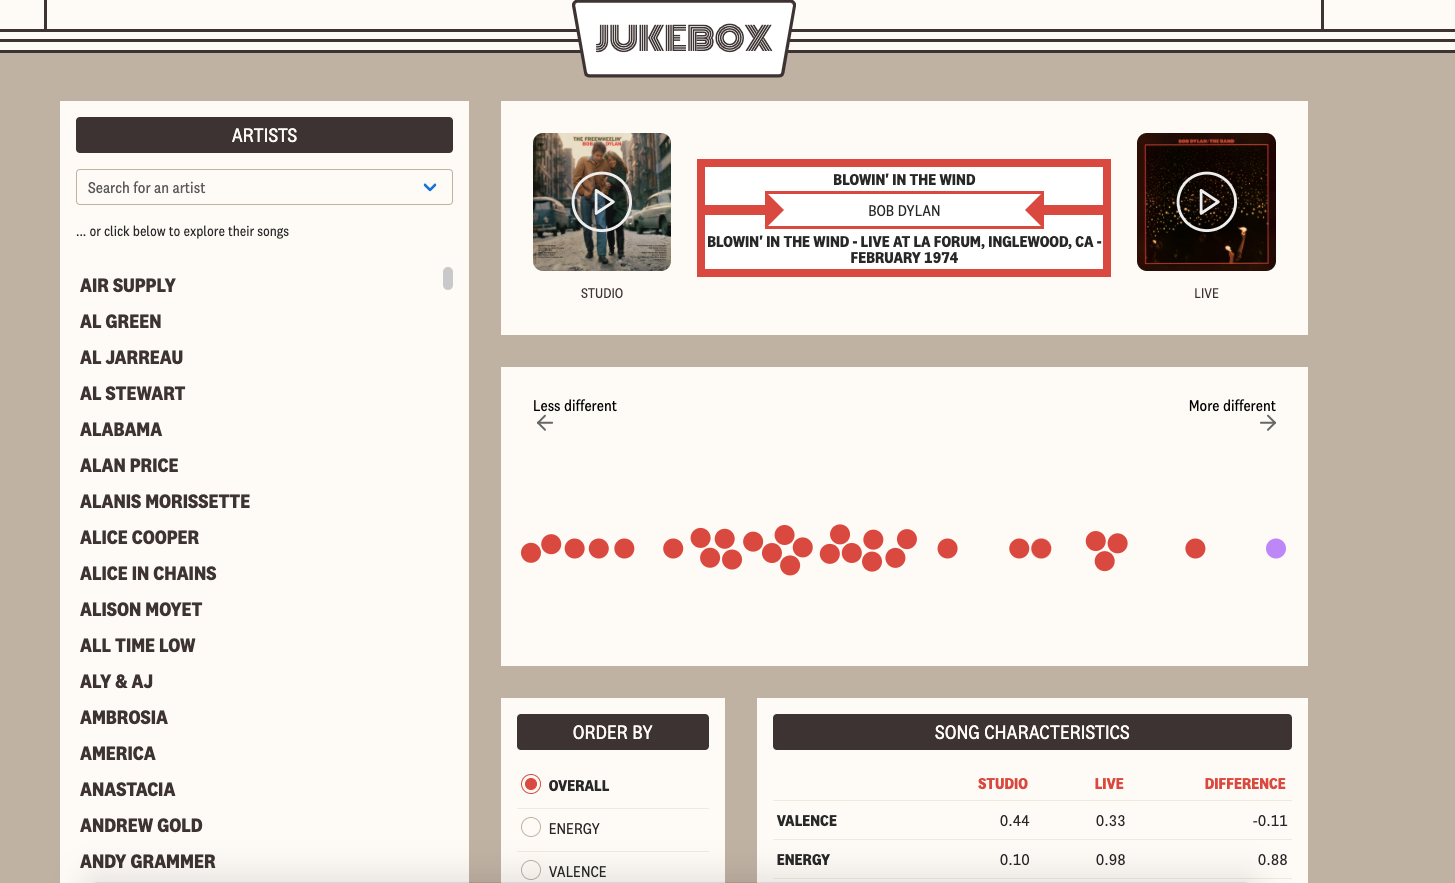
\includegraphics[width=300px,height=200]{images/juke}

\begin{center}\rule{0.5\linewidth}{0.5pt}\end{center}

\hypertarget{absenteeism-in-nyc-public-schools}{%
\paragraph{Absenteeism in NYC Public
Schools}\label{absenteeism-in-nyc-public-schools}}

\begin{longtable}[]{@{}lr@{}}
\toprule
Overview & \\
\midrule
\endhead
\bottomrule
\end{longtable}

NYC public schools vary randomly on whether or not they have the option
of a self-contained classroom for students with special needs. Matching
schools on various demographic variables, I explore the effect of the
self-contained class option on Attendance Rates. Employing propensity
score weighting through IPTW, I create a weighted population in which
the covariate distribution is balanced between treatment groups, and
later use principal stratification to explore heterogeneity in treatment
effect.

\begin{longtable}[]{@{}lr@{}}
\toprule
Technical & \\
\midrule
\endhead
\bottomrule
\end{longtable}

Matching: R (MatchIt, IPTW)

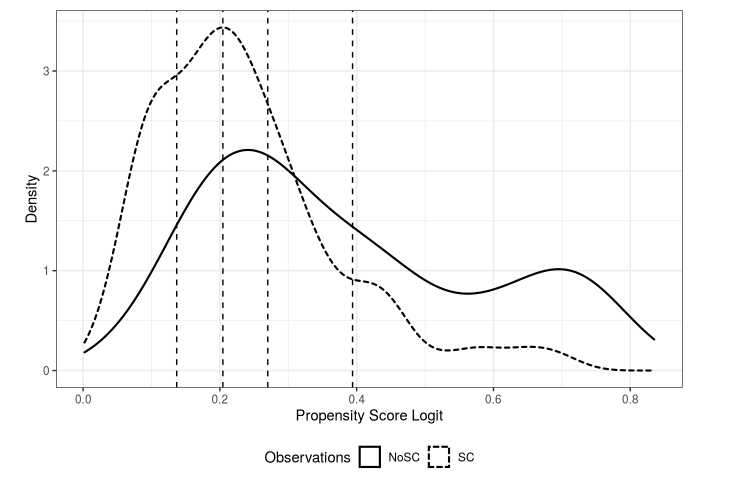
\includegraphics[width=300px,height=200]{images/prop}

\begin{center}\rule{0.5\linewidth}{0.5pt}\end{center}

\hypertarget{random-forest-hospitalization-prediction}{%
\paragraph{Random Forest Hospitalization
Prediction}\label{random-forest-hospitalization-prediction}}

\begin{longtable}[]{@{}lr@{}}
\toprule
Overview & \\
\midrule
\endhead
\bottomrule
\end{longtable}

Central to the debate of ethical algorithm design is a consideration of
mis-classification costs for supervised learning methods. By building in
asymmetric costs through sampling, machine learning engineers can take
heed of policy makers' desired cost-ratios. This random forest algorithm
takes asymmetric sampling into account when predicting death rates of
coronavirus patients in South Korea using the Kaggle COVID-19 Open
Research Dataset.

\begin{longtable}[]{@{}lr@{}}
\toprule
Technical & \\
\midrule
\endhead
\bottomrule
\end{longtable}

Data cleaning: tidyverse Random Forest: R (randomforest) Interactive
Confusion Tables: kableExtra

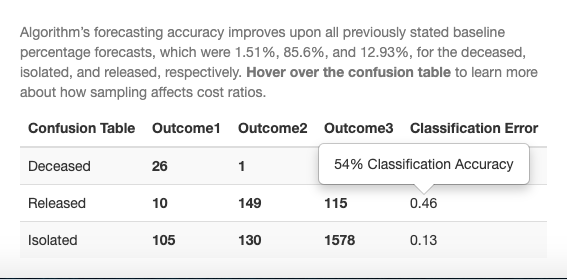
\includegraphics[width=300px,height=200]{images/rf1}

\begin{center}\rule{0.5\linewidth}{0.5pt}\end{center}

\hypertarget{causality-in-teacher-retention}{%
\paragraph{Causality in Teacher
Retention}\label{causality-in-teacher-retention}}

\begin{longtable}[]{@{}lr@{}}
\toprule
Overview & \\
\midrule
\endhead
\bottomrule
\end{longtable}

In experiments where randomization is not feasible, propensity score
matching helps to control for confounded relationships among variables.
Analysts working in this causal framework often run into a particular
issue: sample size affects their ability to arrive at evenly matched
samples. The problem is especially prevalent in observational studies
that use administrative data. In partnernship with the Yale National
Initiative, we evaluate trends in teacher retention across the
Philadelphia School District, and arrive at better percent balance
improvement in our causal model by trimming mis-represented groups.
*data private on github

\begin{longtable}[]{@{}lr@{}}
\toprule
Technical & \\
\midrule
\endhead
\bottomrule
\end{longtable}

Data cleaning: tidyverse Causal Inference: R (MatchIt)

\end{document}
